\documentclass{beamer}
\usepackage{relsize}
\usepackage{color}

\usepackage{listings}
\usetheme{CambridgeUS}
%\usepackage{beamerthemesplit} % new 
\usepackage{enumitem}
\usepackage{amsmath}                    % See geometry.pdf to learn the layout options. 
\usepackage{amsthm}                   % See geometry.pdf to learn the layout options. There 
\usepackage{amssymb}                    % See geometry.pdf to learn the layout options. 
\usepackage[utf8]{inputenc} 
\usepackage{graphicx}
\usepackage[english,bulgarian]{babel}

\lstset{language=C++,
                basicstyle=\ttfamily,
                keywordstyle=\color{blue}\ttfamily,
                stringstyle=\color{red}\ttfamily,
                commentstyle=\color{green}\ttfamily,
                morecomment=[l][\color{magenta}]{\#}
}

\newtheorem{mydef}{Дефиниция}[section]
\newtheorem{lem}{Лема}[section]
\newtheorem{thm}{Твърдение}[section]

\DeclareMathOperator{\restrict}{\upharpoonright}

\setitemize{label=\usebeamerfont*{itemize item}%
  \usebeamercolor[fg]{itemize item}
  \usebeamertemplate{itemize item}}

\setbeamercovered{transparent}



\begin{document}
\title[Обектно ориентирано програмиране]{Динамична памет} 
\author{Калин Георгиев} 
\frame{\titlepage} 

\section{Динамична памет} 


\begin{frame}
\centerline{Динамична памет}
\end{frame}


\begin{frame}[fragile]
\frametitle{Въвеждане на масив}

\begin{flushleft}
\relscale{0.75}
\begin{lstlisting}
long* inputArray (size_t &n)
{ 
   cin >> n;
\end{lstlisting}  
\end{flushleft}

\begin{itemize}
  \item Размерът е определен от подтребителския вход!
\end{itemize}

\begin{flushleft}
\relscale{0.75}
\begin{lstlisting}
  long result[n];
  for (int i = 0; i < n; i++)
    cin >> result[i];

  return result;
}

\end{lstlisting}  
\end{flushleft}

 

\end{frame}


\begin{frame}[fragile]
\frametitle{Изпълнение}

\begin{flushleft}
\relscale{0.75}
\begin{lstlisting}
long* inputArray (size_t &n)
{ 
  cin >> n;
  long result[n];
  for (int i = 0; i < n; i++)
    cin >> result[i];

  return result;
}

int main ()
{
  size_t n;
  long *numbers = inputArray (n);
}

\end{lstlisting}  
\end{flushleft}

 

\end{frame}





\begin{frame}[fragile]
\frametitle{Изпълнение}


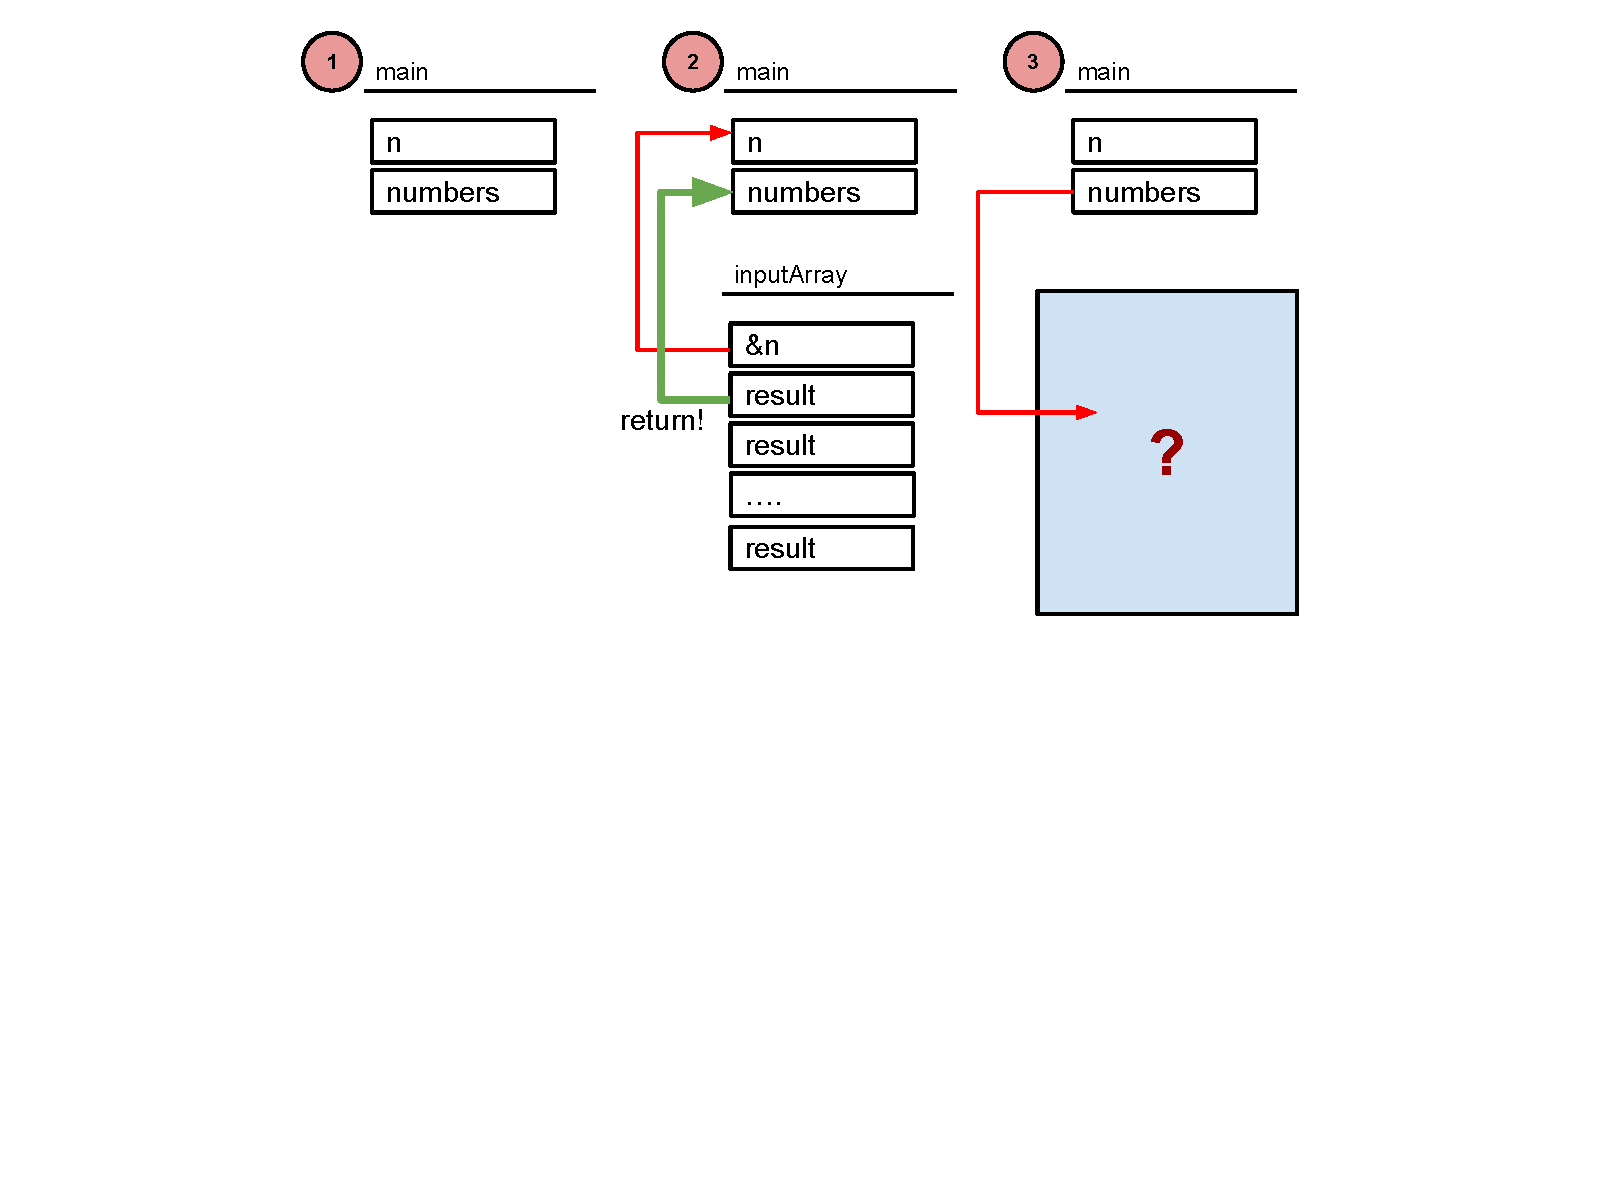
\includegraphics[width=12.5cm]{images/stack}

\vspace{-200px}
\begin{flushleft}
\relscale{0.5}
\begin{lstlisting}
long* inputArray (size_t &n)
{ 
  cin >> n;
  long result[n];
  for (int i = 0; i < n; i++)
    cin >> result[i];

  return result;
}

int main ()
{
  size_t n;
  long *numbers; //(1)
  numbers = inputArray (n); //(2)
  //(3) 
  printArray(numbers,n);
}

\end{lstlisting}  
\end{flushleft}

\end{frame}




\begin{frame}[fragile]
\frametitle{Решение със заделяне на памет в Heap}


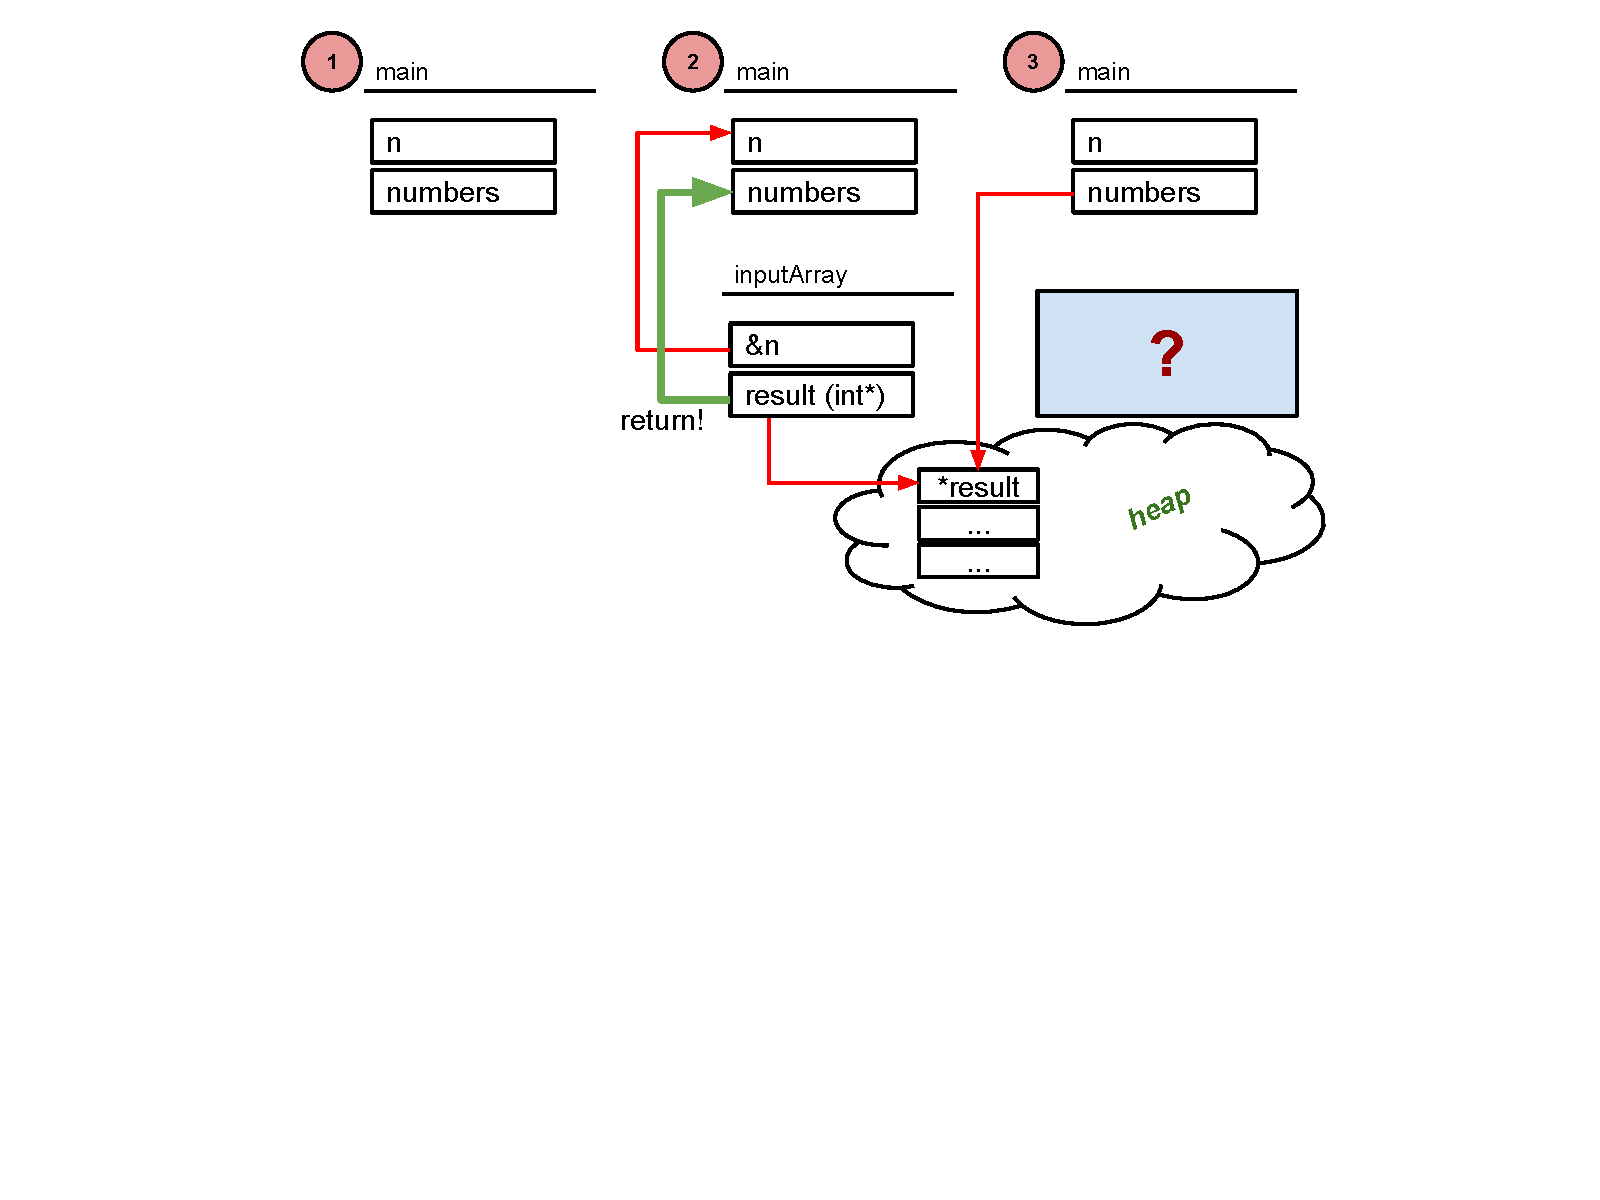
\includegraphics[width=12.5cm]{images/heap}

\vspace{-200px}
\begin{flushleft}
\relscale{0.5}
\begin{lstlisting}
long* inputArray (size_t &n)
{ 
  cin >> n;
  //long* result[n];
  long* result = new long[n];
  for (int i = 0; i < n; i++)
    cin >> result[i];

  return result;
}

int main ()
{
  size_t n;
  long *numbers; //(1)
  numbers = inputArray (n); //(2)
  //(3) 
  printArray(numbers,n);
}

\end{lstlisting}  
\end{flushleft}

\end{frame}



\begin{frame}[fragile]
\frametitle{Stack VS Heap}

\vspace{-10px}
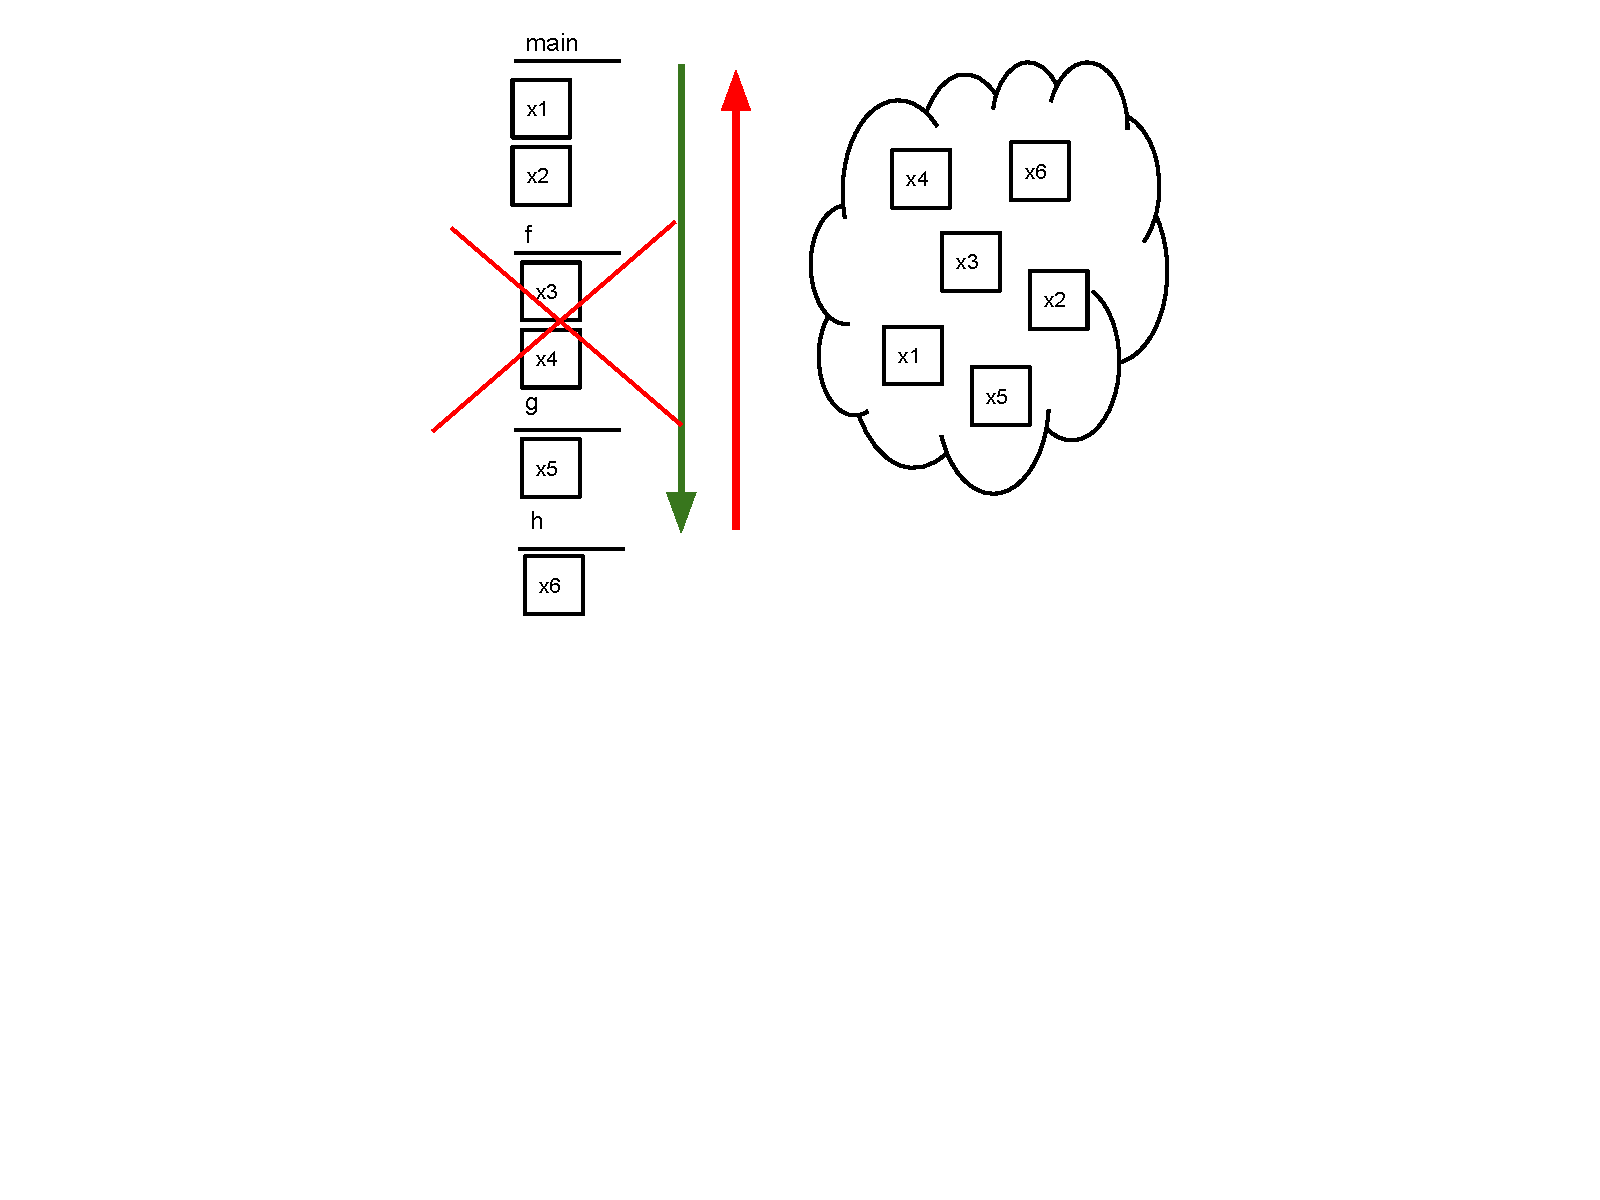
\includegraphics[width=12.5cm]{images/stackVSheap}

\vspace{-150px}


\begin{columns}[t]
  \begin{column}{0.5\textwidth}

\begin{flushleft}
\relscale{0.5}
\begin{lstlisting}
void f (int x3) {int x4;}
void g () {int x5; h(0);}
void h (int x6) {//PAUSE!}
int main ()
{
  int x1,x2;
  f(0); g();
}
\end{lstlisting}  
\end{flushleft}
  \end{column}
  \begin{column}{0.5\textwidth}
\begin{flushleft}
\relscale{0.5}
\begin{lstlisting}
void f (int *x3) {int *x4 = new int;}
void g () {int *x5 = new int; h(new int);}
void h (int *x6) {}
int main ()
{
  int *x1 = new int, *x2 = new int;
  f(new int); g(); //PAUSE!
}
\end{lstlisting}  
\end{flushleft}
  \end{column}
\end{columns}


\end{frame}

\begin{frame}
\centerline{DELETE!}
\end{frame}

\begin{frame}[fragile]
\frametitle{Ръчно освобождаване на ръчно заетата памет}


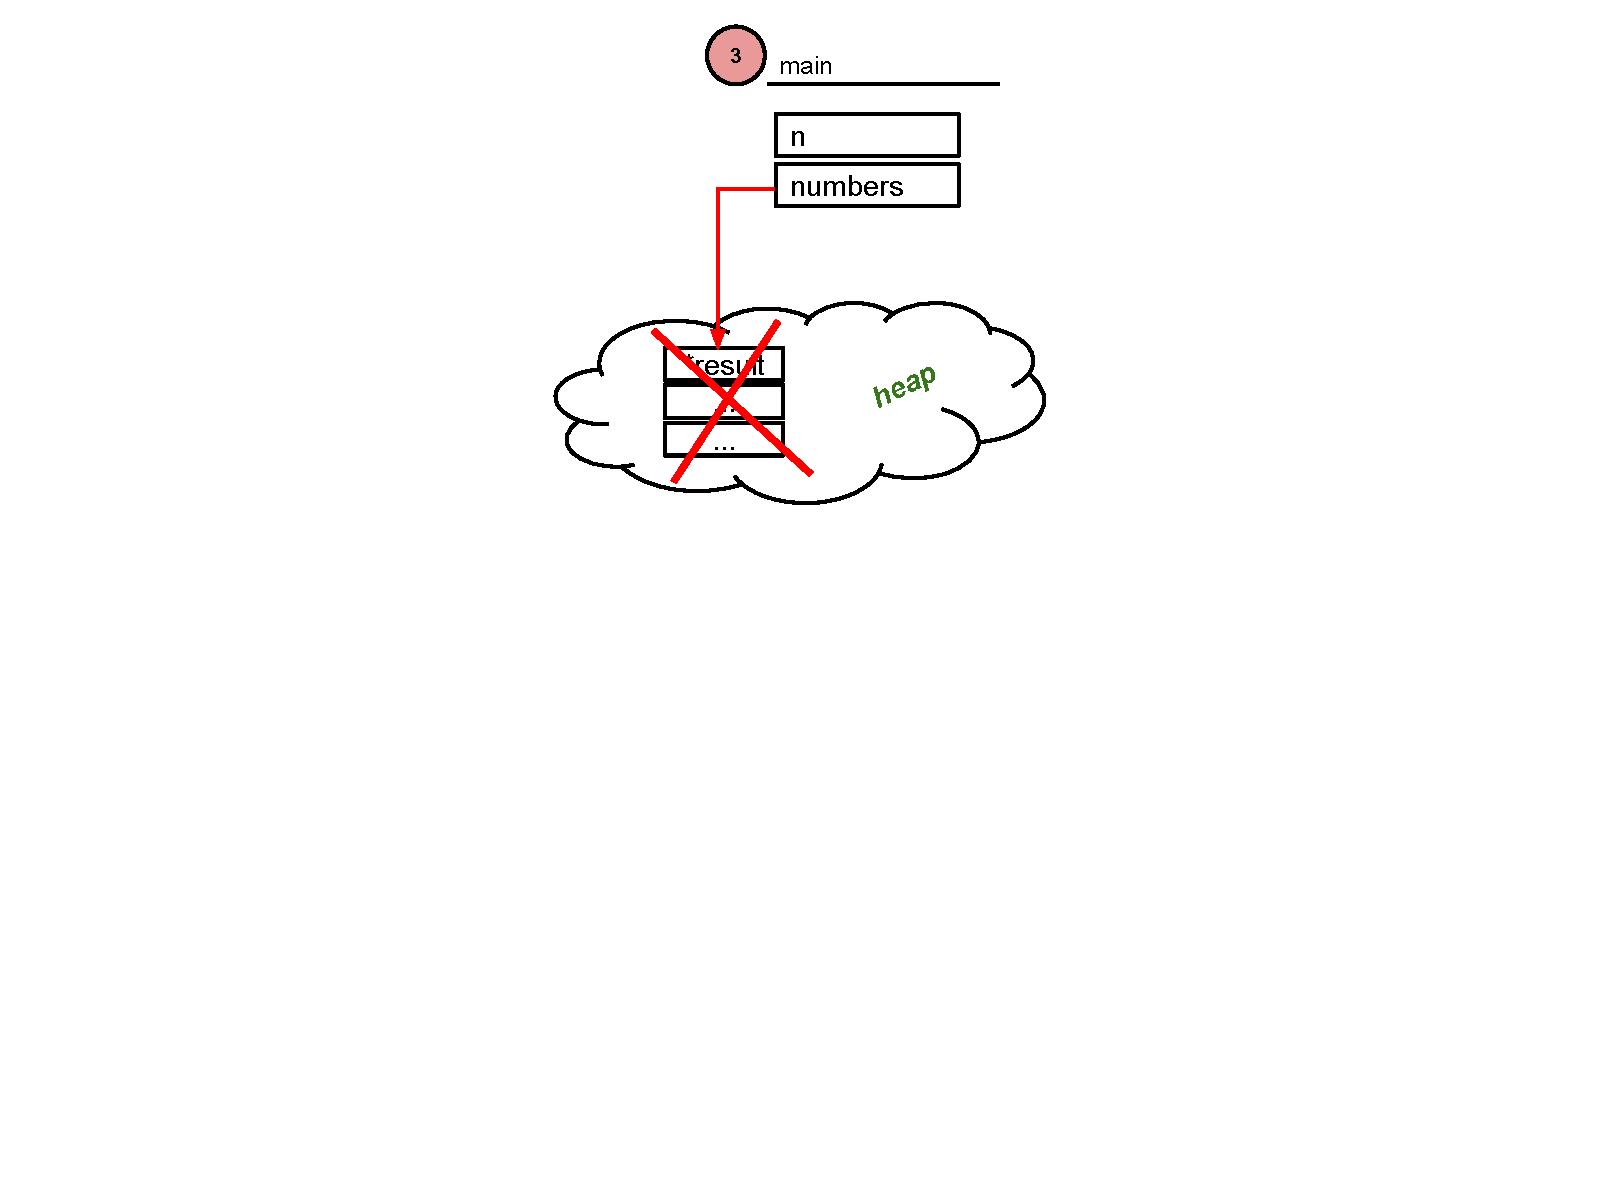
\includegraphics[width=12.5cm]{images/delete}

\vspace{-230px}
\begin{flushleft}
\relscale{0.5}
\begin{lstlisting}
long* inputArray (size_t &n)
{ 
  cin >> n;
  //T result[n];
  long* result = new long[n];
  for (int i = 0; i < n; i++)
    cin >> result[i];

  return result;
}

int main ()
{
  size_t n;
  long *numbers; //(1)
  numbers = inputArray (n); //(2)
  //(3) 
  printArray(numbers,n);
  delete numbers;
} 

\end{lstlisting}  
\end{flushleft}

\end{frame}




\begin{frame}[fragile]
\frametitle{Примери:}

\begin{itemize}
  \item Работа с низове
  \item Обединиение и сечение на елементи на масиви
\end{itemize}


\end{frame}


\begin{frame}
\centerline{Благодаря за вниманието!}
\end{frame}

\end{document}



\begin{columns}[t]
  \begin{column}{0.55\textwidth}

  \end{column}
  \begin{column}{0.45\textwidth}

  \end{column}
\end{columns}
